\documentclass[document.tex]{subfiles} 
\begin{document}

\clearpage

\subsection{Сумматоры}
Сумматор -- устройство, преобразующее информационные сигналы (аналоговые или
цифровые) в сигнал, эквивалентный сумме этих сигналов. Полные сумматоры --
тринарные (трёхоперандные) сумматоры по модулю с разрядом переноса,
характеризующиеся наличием трёх входов, на которые подаются одноимённые разряды
двух складываемых чисел и перенос из предыдущего (более младшего) разряда, и
двумя выходами: на одном реализуется арифметическая сумма по модулю в данном
разряде, а на другом — перенос в следующий (более старший
разряд)~\cite{wikiadder}.

Вся кодовая база сумматоров находится в пакете devices.adder и наследуется от
абстрактного класса Device.

\clearpage
\subsubsection{Параллельный сумматор}

Параллельный (многоразрядный) сумматор можно описать следующим образом:
\begin{equation}
\label{eq:adders}
\forall x: A_x = F_x \oplus S_x \oplus C_{x - 1} 
\end{equation}

\begin{equation}
\label{eq:adderp}
\forall x: C_x = (F_x \wedge S_x) \vee (F_x \wedge C_{x - 1}) \vee (S_x \wedge
C_{x - 1}) 
\end{equation}

\begin{equation}
\label{eq:addero}
\forall y: O_y = \begin{cases}
A_y &\mbox{при } y < n; \\
C_{y - 1} &\mbox{при } y \equiv n; \\
C_{y - 2} \oplus C_{y - 1} &\mbox{при } y \equiv n + 1.
\end{cases} 
\end{equation}

В выражениях~\ref{eq:adders},~\ref{eq:adderp}~и~\ref{eq:addero}:
\begin{itemize}[noitemsep]
  \item $x$ -- индекс входного разряда первого и второго операнда;
  \item $y$ -- индекс выходного разряда;
  \item $n$ -- количество входных разрядов первого и второго операнда;
  \item $F$ -- набор входных разрядов первого операнда;
  \item $S$ -- набор входных разрядов второго операнда;
  \item $C$ -- разряды переноса;
  \item $A$ -- разряды суммы;
  \item $O$ -- выходные разряды сумматора.
\end{itemize}

\clearpage

Основным классом, реализующим функционал сумматора (характерной особенностью
которого является возможность генерации двух дополнительных выходных сигналов --
переноса и переполнения), является DeviceAdd. Описание сумматора в
разрабатываемой библиотеке представлено в листинге~\ref{lst:adder}.

\begin{listing}[ht]
\begin{minted}[linenos=true]{python}
class DeviceAdd(Device):
    """Adder device"""
    mandatory_signals = ('strobe_signals', 'first_signals', 
                         'second_signals', 'output_signals',)
    mandatory_signals_using_subs = ('strobe_signals',)
    truth_table_signals = ('strobe_signals', 'first_signals', 
                           'second_signals', 'output_signals',)
    constraints = {
        'strobe_signals': {
            'min': 1,
            'max': 10
        },
        'first_signals': {
            'min': 1,
            'max': 5
        },
        'second_signals': {
            'min': 1,
            'max': 5
        },
        'output_signals': {
            'min': 1,
            'max': 7
        }
    }
\end{minted}
\caption{Программное описание класса сумматора}
\label{lst:adder}
\end{listing}

В листинге~\ref{lst:addergen} представлен код для программного синтеза
параллельного сумматора с 2 входными разрядами первого операнда
(first\_signals='f:2'), 2 входными разрядами второго операнда
(second\_signals='s:2'), 1 прямым входным разрядом строб-сигнала
(strobe\_signals='z:1') и 4 выходными разрядами (output\_signals='o:4').

\clearpage

\begin{listing}[ht]
\begin{minted}{pycon}
>>> from circuitry.devices.adder import DeviceAdd        
>>> pprint(                                                   
...     DeviceAdd(strobe_signals='z:1', first_signals='a:2',
...               second_signals='s:2', output_signals='o:4',
...               strobe_signals_subs=dict(z0=1))         
... )
{'first_signals': (a0, a1),
 'functions': [And(Or(And(Not(a0), s0), 
                      And(Not(s0), a0)), z0),
               And(Or(And(Not(a1), Or(And(Not(s1), a0, s0), 
                                      And(Or(Not(a0), Not(s0)), s1))), 
                      And(Or(And(a0, s0), Not(s1)), 
                          Or(Not(a0), Not(s0), s1), a1)), z0), 
               And(Or(And(a0, a1, s0), And(a0, s0, s1), 
                      And(a1, s1)), z0),
               And(Or(And(Or(And(a0, a1, s0), 
                             And(a0, s0, s1), And(a1, s1)), 
                          Or(Not(a0), Not(s0))), 
                      And(Or(Not(a0), Not(a1),
                             Not(s0)), 
                          Or(Not(a0), Not(s0), Not(s1)),
                          Or(Not(a1), Not(s1)), a0, s0)), z0)], 
 'output_signals': (o0, o1, o2, o3),
 'second_signals': (s0, s1),
 'strobe_signals': (z0,),
 'strobe_signals_function': z0,
 'strobe_signals_subs': {'z0': 1},
 'strobe_signals_truth_table': [1],
 'truth_table': [([1], [0, 0], [0, 0], [0, 0, 0, 0]),
                 ([1], [0, 0], [1, 0], [1, 0, 0, 0]),
                 ([1], [0, 0], [0, 1], [0, 1, 0, 0]),
                 ([1], [0, 0], [1, 1], [1, 1, 0, 0]),
                 ([1], [1, 0], [0, 0], [1, 0, 0, 0]),
                 ([1], [1, 0], [1, 0], [0, 1, 0, 1]),
                 ([1], [1, 0], [0, 1], [1, 1, 0, 0]),
                 ([1], [1, 0], [1, 1], [0, 0, 1, 0]),
                 ([1], [0, 1], [0, 0], [0, 1, 0, 0]),
                 ([1], [0, 1], [1, 0], [1, 1, 0, 0]),
                 ([1], [0, 1], [0, 1], [0, 0, 1, 1]),
                 ([1], [0, 1], [1, 1], [1, 0, 1, 1]),
                 ([1], [1, 1], [0, 0], [1, 1, 0, 0]),
                 ([1], [1, 1], [1, 0], [0, 0, 1, 0]),
                 ([1], [1, 1], [0, 1], [1, 0, 1, 1]),
                 ([1], [1, 1], [1, 1], [0, 1, 1, 0])]}
\end{minted}
\caption{Программный синтез сумматора}
\label{lst:addergen}
\end{listing}

\clearpage

На рисунке~\ref{fig:deviceadder} представлено условно-графическое обозначение
синтезированного сумматора.

\begin{figure}[here]
\centering
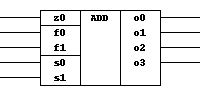
\includegraphics{devices_adder_sym}
\caption{Условно-графическое обозначение сумматора}
\label{fig:deviceadder}
\end{figure}

На рисунке~\ref{fig:deviceaddermat} представлено устройство
синтезированного сумматора в виде модели Simulink.

\begin{figure}[here]
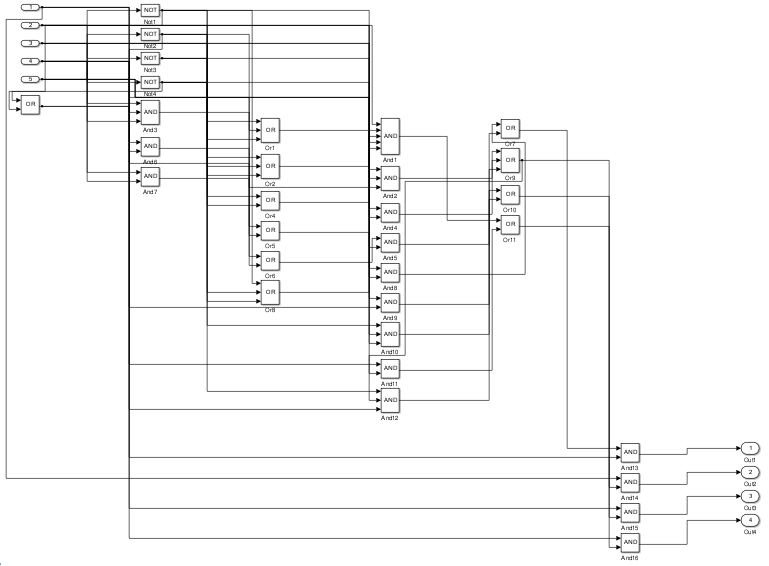
\includegraphics[width=1\linewidth]{devices_adder_mat}
\caption{Представление сумматора в виде модели Simulink}
\label{fig:deviceaddermat}
\end{figure}

\clearpage
\subsubsection{Устройство инкремента}

Устройство инкремента описывается следующим образом на базе параллельного
сумматора с использованием формул из
выражений~\ref{eq:adders},~\ref{eq:adderp}~и~\ref{eq:addero}:
\begin{equation}
\label{eq:incf}
\forall x: F_x = D_x 
\end{equation}

\begin{equation}
\label{eq:incs}
\forall x: S_x = \begin{cases}
1 &\mbox{при } x \equiv 0; \\
0 &\mbox{при } x > 0.
\end{cases}
\end{equation}

В выражениях~\ref{eq:incf},~и~\ref{eq:incs}:
\begin{itemize}[noitemsep]
  \item $x$ -- индекс входного разряда устройства инкремента;
  \item $D$ -- набор входных разрядов устройства инкремента;
  \item $F$ -- набор входных разрядов первого операнда сумматора;
  \item $S$ -- набор входных разрядов второго операнда сумматора;
\end{itemize}

\clearpage

Описание устройства инкремента в разрабатываемой библиотеке представлено в
листинге~\ref{lst:inc}.

\begin{listing}[ht]
\begin{minted}[linenos=true]{python}
class DeviceInc(Device):
    """Increment device"""
    mandatory_signals = ('strobe_signals', 'data_signals', 'output_signals',)
    mandatory_signals_using_subs = ('strobe_signals',)
    truth_table_signals = ('strobe_signals', 'data_signals', 'output_signals',)
    constraints = {
        'strobe_signals': {
            'min': 1,
            'max': 10
        },
        'data_signals': {
            'min': 1,
            'max': 5
        },
        'output_signals': {
            'min': 1,
            'max': 7
        }
    }
\end{minted}
\caption{Программное описание класса инкремента}
\label{lst:inc}
\end{listing}

\clearpage
В листинге~\ref{lst:incgen} представлен код для программного синтеза
устройства инкремента с 2 входными разрядами данных (data\_signals='d:2'), 1
прямым входным разрядом строб-сигнала (strobe\_signals='z:1') и 2 выходными
разрядами (output\_signals='o:2').

\begin{listing}[ht]
\begin{minted}{pycon}
>>> from circuitry.devices.adder import DeviceInc             
>>> pprint(                                                 
...     DeviceInc(strobe_signals='z:1', data_signals='a:2',
...               output_signals='o:2', strobe_signals_subs=dict(z0=1))
... )
{'data_signals': (a0, a1),
 'functions': [And(Not(a0), z0),
               And(Or(And(Not(a0), a1), And(Not(a1), a0)), z0)],
 'output_signals': (o0, o1),
 'strobe_signals': (z0,),
 'strobe_signals_function': z0,
 'strobe_signals_subs': {'z0': 1},
 'strobe_signals_truth_table': [1],
 'truth_table': [([1], [0, 0], [1, 0]),
                 ([1], [1, 0], [0, 1]),
                 ([1], [0, 1], [1, 1]),
                 ([1], [1, 1], [0, 0])]}
\end{minted}
\caption{Программный синтез устройства инкремента}
\label{lst:incgen}
\end{listing}

На рисунке~\ref{fig:deviceinc} представлено условно-графическое обозначение
синтезированного устройства инкремента.

\begin{figure}[here]
\centering
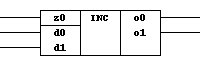
\includegraphics{devices_inc_sym}
\caption{Условно-графическое обозначение устройства инкремента}
\label{fig:deviceinc}
\end{figure}

\clearpage

На рисунке~\ref{fig:deviceincmat} представлено устройство
синтезированного инкремента в виде модели Simulink.

\begin{figure}[here]
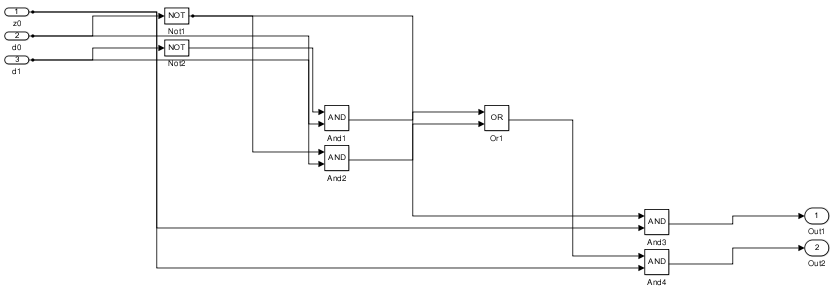
\includegraphics[width=1\linewidth]{devices_inc_mat}
\caption{Представление инкремента в виде модели Simulink}
\label{fig:deviceincmat}
\end{figure}

\clearpage
\subsubsection{Устройство декремента}

Устройство декремента описывается следующим образом на базе параллельного
сумматора с использованием формул из
выражений~\ref{eq:adders},~\ref{eq:adderp}~и~\ref{eq:addero}:
\begin{equation}
\label{eq:decf}
\forall x: F_x = D_x 
\end{equation}

\begin{equation}
\label{eq:decs}
\forall x: S_x = 1
\end{equation}

В выражениях~\ref{eq:decf},~и~\ref{eq:decs}:
\begin{itemize}[noitemsep]
  \item $x$ -- индекс входного разряда устройства декремента;
  \item $D$ -- набор входных разрядов устройства декремента;
  \item $F$ -- набор входных разрядов первого операнда сумматора;
  \item $S$ -- набор входных разрядов второго операнда сумматора;
\end{itemize}

\clearpage

Описание устройства инкремента в разрабатываемой библиотеке представлено в
листинге~\ref{lst:dec}.

\begin{listing}[ht]
\begin{minted}[linenos=true]{python}
class DeviceDec(Device):
    """Decrement device"""
    mandatory_signals = ('strobe_signals', 'data_signals', 'output_signals',)
    mandatory_signals_using_subs = ('strobe_signals',)
    truth_table_signals = ('strobe_signals', 'data_signals', 'output_signals',)
    constraints = {
        'strobe_signals': {
            'min': 1,
            'max': 10
        },
        'data_signals': {
            'min': 1,
            'max': 5
        },
        'output_signals': {
            'min': 1,
            'max': 7
        }
    }
\end{minted}
\caption{Программное описание класса декремента}
\label{lst:dec}
\end{listing}

\clearpage
В листинге~\ref{lst:decgen} представлен код для программного синтеза
устройства декремента с 2 входными разрядами данных (data\_signals='d:2'), 1
прямым входным разрядом строб-сигнала (strobe\_signals='z:1') и 2 выходными
разрядами (output\_signals='o:2').

\begin{listing}[ht]
\begin{minted}{pycon}
>>> from circuitry.devices.adder import DeviceDec          
>>> pprint(                                                
...     DeviceDec(strobe_signals='z:1', data_signals='a:2',
...               output_signals='o:2', strobe_signals_subs=dict(z0=1))
... )
{'data_signals': (a0, a1),
 'functions': [And(Not(a0), z0), And(Or(Not(a0), a1), Or(Not(a1), a0), z0)],
 'output_signals': (o0, o1),
 'strobe_signals': (z0,),
 'strobe_signals_function': z0,
 'strobe_signals_subs': {'z0': 1},
 'strobe_signals_truth_table': [1],
 'truth_table': [([1], [0, 0], [1, 1]),
                 ([1], [1, 0], [0, 0]),
                 ([1], [0, 1], [1, 0]),
                 ([1], [1, 1], [0, 1])]}
\end{minted}
\caption{Программный синтез устройства декремента}
\label{lst:decgen}
\end{listing}

На рисунке~\ref{fig:devicedec} представлено условно-графическое обозначение
синтезированного устройства декремента.

\begin{figure}[here]
\centering
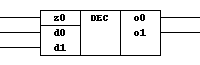
\includegraphics{devices_dec_sym}
\caption{Условно-графическое обозначение устройства декремента}
\label{fig:devicedec}
\end{figure}

\clearpage

На рисунке~\ref{fig:devicedecmat} представлено устройство
синтезированного декремента в виде модели Simulink.

\begin{figure}[here]
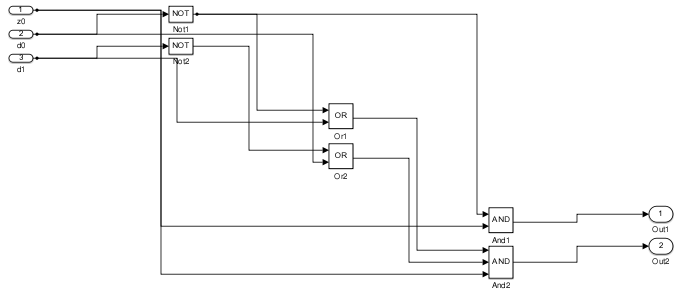
\includegraphics[width=1\linewidth]{devices_dec_mat}
\caption{Представление декремента в виде модели Simulink}
\label{fig:devicedecmat}
\end{figure}

\clearpage
\subsubsection{Устройство отрицания в дополнительном коде}

Устройство отрицания в дополнительном коде описывается следующим образом на базе
двух устройств поразрядной инверсии, устройства инкремента и устройства
декремента с использованием формул из
выражений~\ref{eq:not},~\ref{eq:incf},~\ref{eq:incs},~\ref{eq:decf}~и~\ref{eq:decs}:
\begin{equation}
\label{eq:nego}
\forall x: O_x = \begin{cases}
inc_{x}(\overline{D}) & \mbox{при } D_{n-1} \equiv 0; \\
\overline{dec_{x}(D)} & \mbox{при } D_{n-1} \equiv 1.
\end{cases} 
\end{equation}

В выражении~\ref{eq:nego}:
\begin{itemize}[noitemsep]
  \item $x$ -- индекс входного разряда устройства отрицания;
  \item $n$ -- количество входных разрядов устройства отрицания;
  \item $inc$ -- функция устройства инкремента;
  \item $dec$ -- функция устройства декремента;
  \item $D$ -- набор входных разрядов устройства отрицания;
\end{itemize}

\clearpage

Описание устройства отрицания в разрабатываемой библиотеке представлено в
листинге~\ref{lst:neg}.

\begin{listing}[ht]
\begin{minted}[linenos=true]{python}
class DeviceNeg(Device):
    """Negation for two's complement"""
    mandatory_signals = ('strobe_signals', 'data_signals', 'output_signals',)
    mandatory_signals_using_subs = ('strobe_signals',)
    truth_table_signals = ('strobe_signals', 'data_signals', 'output_signals',)
    constraints = {
        'strobe_signals': {
            'min': 1,
            'max': 10
        },
        'data_signals': {
            'min': 1,
            'max': 5
        },
        'output_signals': {
            'min': 1,
            'max': 5
        }
    }
\end{minted}
\caption{Программное описание устройства отрицания}
\label{lst:neg}
\end{listing}

\clearpage
В листинге~\ref{lst:neggen} представлен код для программного синтеза
устройства отрицания в дополнительном коде с 2 входными разрядами данных
(data\_signals='d:2'), 1 прямым входным разрядом строб-сигнала
(strobe\_signals='z:1') и 2 выходными разрядами (output\_signals='o:2').

\begin{listing}[ht]
\begin{minted}{pycon}
>>> from circuitry.devices.adder import DeviceNeg          
>>> pprint(                                                
...     DeviceNeg(strobe_signals='z:1', data_signals='d:2',
...               output_signals='o:2', strobe_signals_subs=dict(z0=1))
... )
{'data_signals': (d0, d1),
 'functions': [And(Or(And(Not(d1), Or(Not(z0), d0)), And(d0, d1, z0)), z0),
               And(Or(And(Not(d1), Or(And(Not(d0), d1), 
                                      And(Not(d1), d0), Not(z0))), 
                      And(Or(And(Not(d0), d1), And(Not(d1), d0)), d1, z0)), 
                      z0)], 
 'output_signals': (o0, o1),
 'strobe_signals': (z0,),
 'strobe_signals_function': z0,
 'strobe_signals_subs': {'z0': 1},
 'strobe_signals_truth_table': [1],
 'truth_table': [([1], [0, 0], [0, 0]),
                 ([1], [1, 0], [1, 1]),
                 ([1], [0, 1], [0, 1]),
                 ([1], [1, 1], [1, 0])]}
\end{minted}
\caption{Программный синтез устройства отрицания}
\label{lst:neggen}
\end{listing}

На рисунке~\ref{fig:deviceneg} представлено условно-графическое обозначение
синтезированного устройства отрицания в дополнительном коде.

\begin{figure}[here]
\centering
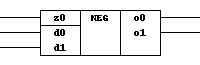
\includegraphics{devices_neg_sym}
\caption{Условно-графическое обозначение устройства отрицания}
\label{fig:deviceneg}
\end{figure}

\clearpage

На рисунке~\ref{fig:devicenegmat} представлено устройство
синтезированного отрицания в виде модели Simulink.

\begin{figure}[here]
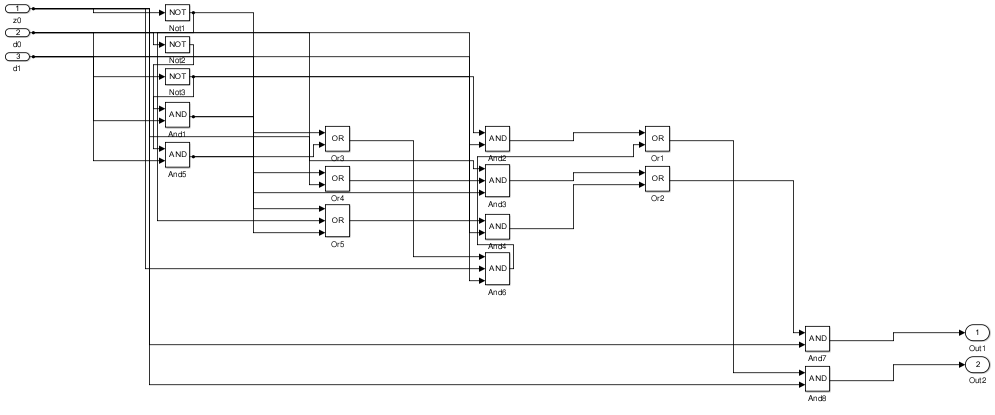
\includegraphics[width=1\linewidth]{devices_neg_mat}
\caption{Представление отрицания в виде модели Simulink}
\label{fig:devicenegmat}
\end{figure}

\end{document}